\documentclass{article}
\usepackage{amsmath}
\usepackage{amssymb}
\usepackage{graphicx}
\usepackage{hyperref}
\usepackage[version=4]{mhchem}

\title{Problem 8}
\date{}

\begin{document}
\maketitle

\section*{Problem}
As shown in the figure, \(A B / / C D . A D \perp A B . A D\) and \(B C\) meet at \(E\) such that \(E B=2 A C\). Show that \(\angle A C D=3 \angle B C D\).\\
\centering
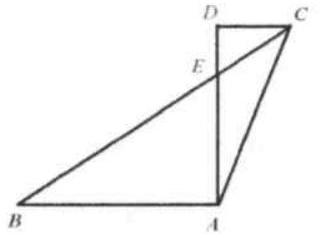
\includegraphics[width=\textwidth]{images/016(2).jpg}

\section*{Solution}
Draw \(A F\), the median of right triangle \(B A E\). Since \(A F\) is the median, by Theorem 1.3, \(A F=B F=N C\).\\
Thus \(A F=A C\).\\
Thus both triangles \(A F B\) and \(C A F\) are isosceles triangles.\\
\centering
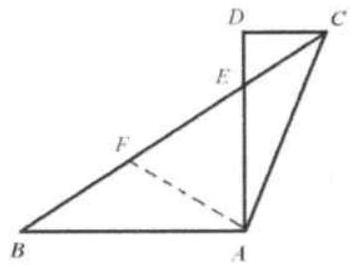
\includegraphics[width=\textwidth]{images/020(3).jpg}

Let \(\angle B=\angle F A B=\alpha\).\\
\(\angle C F A\) is the exterior angle of triangle \(A B F\). So \(\angle C F A=\) \(\angle A C F=2 \alpha\).\\
Since \(A B / / C D, \angle B=\angle D C E=\alpha\).\\
\(\angle A C D=\angle A C F+\angle D C E=3 \alpha=3 \angle B C D\).\\
\centering
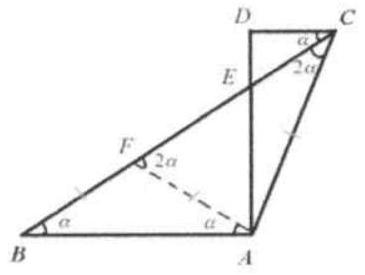
\includegraphics[width=\textwidth]{images/020(2).jpg}

\end{document}
